

We present examples of intervention where an \textit{opportunistic adversary} acts in the environment to disrupt a user from reaching a desirable goal state $G_d$. In the computer security literature, the opportunistic adversary is identified as one that is flexible about the plan of attack and continuously looks for opportunities to cause an undesirable state rather than strategically planning attacks. \cite{Zhang2014opportunistic}. 
In this paper, we model situations where (1) the attack opportunities are available in the environment apriori (e.g., hidden pothole on a path) and (2) opportunistic adversary actively engages in creating attacks during the user's plan execution (e.g., repeatedly sending different phishing emails, hoping the user would eventually fall for one). Regardless the attack type, from the perspective of the observer, some actions in the environment may just be nuisances or for the user (e.g., receiving many phishing email) or common harmless actions (e.g., logging in to email). On the other hand, certain action sequences may lead the user unwittingly towards an undesirable state $G_u$ (e.g., actually opening a phishing email and clicking the link).  We refer to the actions that will lead the user toward $G_u$ as \textit{critical action}s. In both cases, the observer monitors the actions and helps the user reach $G_d$ safely by intervening when critical actions are observed. 
%The user computes a plan for a desirable goal state, $G_d$. Given the unexpected modification to the domain, executing this precompiled plan may likely cause the user to reach the undesirable state ($G_u$).

\textbf{Hidden Attack Opportunities}: We chose a grid navigation example to model intervention when there is a hidden attack opportunity. On a 4x4 grid shown in Figure \ref{fig:single}, an agent U navigates by moving vertically and horizontally to reach a desired goal $G_d$. Initially, U is on cell (1,1) and  cell (3,3) has a pit U can not see, but would like to avoid. For simplicity, let us assume U is optimal and will always choose the shortest path to reach $G_d$. Given U's initial position, plans A, B and C are all feasible solutions for U. However, the hidden pit yields plans B and C unsafe as they lead to the undesirable state ($G_u$). The observer agent monitors U's actions in the domain and intervenes for the benefit of U. The black dots show critical actions the observer must recognize. Actions \texttt{MOVE CELL\_2\_3 CELL\_3\_3} and \texttt{MOVE CELL\_3\_2 CELL\_3\_3} are clearly critical because they directly lead U to the pit. A less obvious critical action is \texttt{MOVE CELL\_2\_1 CELL\_3\_1}. This is because, from that position U can only move up to reach $G_d$ without violating optimality. If the observer interrupted U prior to observing the critical actions, they will be treated as false alarms.

\textbf{Active Opportunistic Adversary}: 
We model an active opportunistic adversary who attempts to make the user reach the undesirable state by leveraging the user's progress. We use the IPC block-words domain  \cite{gupta1992bw}. Figure \ref{fig:multi} shows states the observer may perceive as the user and the attacker execute actions to spell different words. Time flows from left to right. Figure \ref{fig:multi} (A) models a  scenario where 4 blocks: T, B, A, D are on the table. User's executes a plan to reach  TAD $ =G_d$, while BAD $ =G_u$. The user can not recognize block B (indicated by dotted lines), and therefore fails to circumvent $G_u$ on his own where the attacker exploits the opportunity of having block A on block D and the hidden block to reach $G_u$. Therefore, assuming both the user and the attacker are optimal, the observer must intervene when \texttt{PICK-UP B} is observed. Any subsequent action must also be flagged if it leads further toward $G_u$ (e.g., \texttt{STACK B A}). Figure \ref{fig:multi} (B) models a similar situation where CUP $ =G_d$ and CUT $ =G_u$. In this case, the observer must intervene when \texttt{STACK T P} is observed. This is because the user is unable to recognize block T and placing U on T (thinking P is free) will make the user unwittingly reach $G_u$. The difference in Figure \ref{fig:multi}(B) is that the critical action is observed earlier compared to \ref{fig:multi}(A). Further, any subsequent action leading  to $G_u$ must also be flagged to prevent aggregating the error.
\begin{figure*}[ht]
        \centering{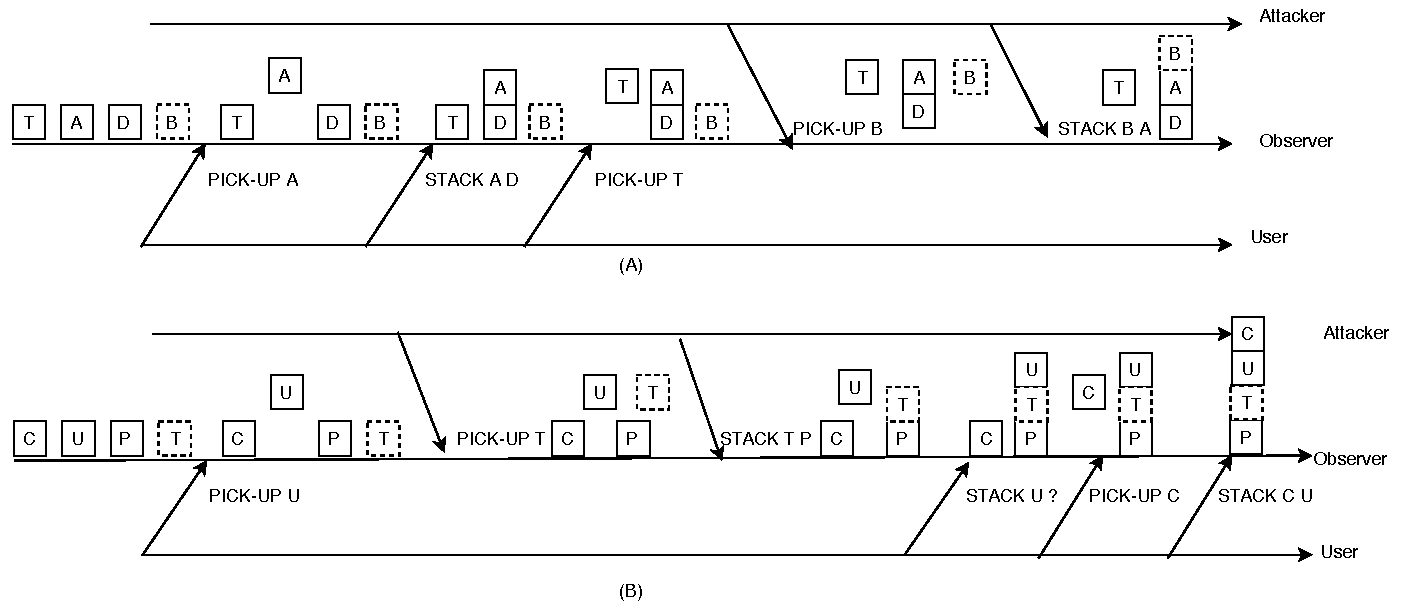
\includegraphics[width=0.7\textwidth]{multi.pdf}}
        \caption{Reaching $G_u$ with an active opportunistic attacker}
        \label{fig:multi}
\end{figure*}
%Figure \ref{fig:example} (right)  illustrates how the user's plans to reach $G_d$ could fail. In this case, given the assumption that the attacker does not backtrack to a previous state and only leverages progress made thus far, it can make four attempts to prevent the user from reaching $G_u$ by inserting the hidden block into the partially built stack. If the user achieves goal states 1 or 4 the user wins despite the attacker. If the observed actions indicate that the user is heading toward one of these two states, then an interrupt is unwarranted. State 3 is less ideal for the user but $G_u$ is not achieved. In state 2 the attacker has successfully reached $G_u$. Observations indicating state 2 warrant interruption.


